% exercise sheet with header on every page for math or close subjects
\documentclass[12pt]{article}
\usepackage[utf8]{inputenc}
\usepackage{latexsym}
\usepackage{multicol}
\usepackage{fancyhdr}
\usepackage{amsfonts}
\usepackage{amsmath}
\usepackage{amssymb}
\usepackage{enumerate}
\usepackage{listings}
\usepackage{graphicx}

% Shortcuts for bb, frak and cal letters
\newcommand{\E}{\mathbb{E}}
\newcommand{\V}{\mathbb{V}}
\renewcommand{\P}{\mathbb{P}}
\newcommand{\N}{\mathbb{N}}
\newcommand{\R}{\mathbb{R}}
\newcommand{\C}{\mathbb{C}}
\newcommand{\Z}{\mathbb{Z}}
\newcommand{\Pfrak}{\mathfrak{P}}
\newcommand{\Pfrac}{\mathfrak{P}}
\newcommand{\Bfrac}{\mathfrak{P}}
\newcommand{\Bfrak}{\mathfrak{B}}
\newcommand{\Fcal}{\mathcal{F}}
\newcommand{\Ycal}{\mathcal{Y}}
\newcommand{\Bcal}{\mathcal{B}}
\newcommand{\Acal}{\mathcal{A}}

% formating
\topmargin -3.5cm
\textheight 22cm
\textwidth 16.0 cm
\oddsidemargin -0.1cm

% Fancy Header on every Page
\pagestyle{fancy}
\lhead{\textbf{Embedded Systems Problem Set B}}
\rhead{Daniel Schäfer (2549458)\\ Rafael Dewes (2548365)\\ Kevin M\"uller (2550062)}
\renewcommand{\headrulewidth}{1.2pt}
\setlength{\headheight}{110pt}

\begin{document}
\pagenumbering{gobble}
\lstset{language=C++}


\section*{Problem B1}
% TODO
\begin{enumerate}[a)]
	\item According to sampling theory (Nyquist criterion) the sampling rate needs to be at least twice as big as the highest frequency of the component sine waves.
	$$ f_s > 2 * f_N$$
	To compute the necessary sampling rate, the Nyquist frequency $f_N$ has to be computed as follows
	$$ S(t) = \underbrace{sin(2\pi t + \frac{1}{4})}_{f = 1Hz} + \underbrace{sin(4\pi t + \frac{1}{4})}_{f = 2Hz}$$
	The highest frequency of the component sine waves is $2$, which means that $f_N = 2$.

	$\Rightarrow$ The signal has to be sampled at least 4 times per second to enable a reconstruction.

	\item Shannon-Whittaker interpolation:
	As calculated above we have a frequency of 4, giving us f = 4.
	We can then define our sinc function in the following way
	\[
    		sinc(i)=
		\begin{cases}
    			 \frac{sin(4{\pi}i)}{4{\pi}i},& \text{if } i\neq 0\\
    			1,              & \text{otherwise}
		\end{cases}
	\]
    Given a reconstruction intervall of [0,2] and a sampling frequency of $f=\frac{1}{4}$ we know that we have 8 samples for this intervall. This gives us the Shannon-Whittaker interpolation function as:

	$$z(t) = \sum_{s=1}^{8} y(t_s) * sinc(t-t_s)$$
	$$=  y(t_1) * sinc(t-t_1) + y(t_2) * sinc(t-t_2) + ...$$
	$$=  y(0) * sinc(t-0) + y(0.25) * sinc(t-0.25) + ...$$

The resulting function {z(t)} gives us a reconstruction of the original signal based on the sampled values plotted as a step function.\\


\begin{centering}
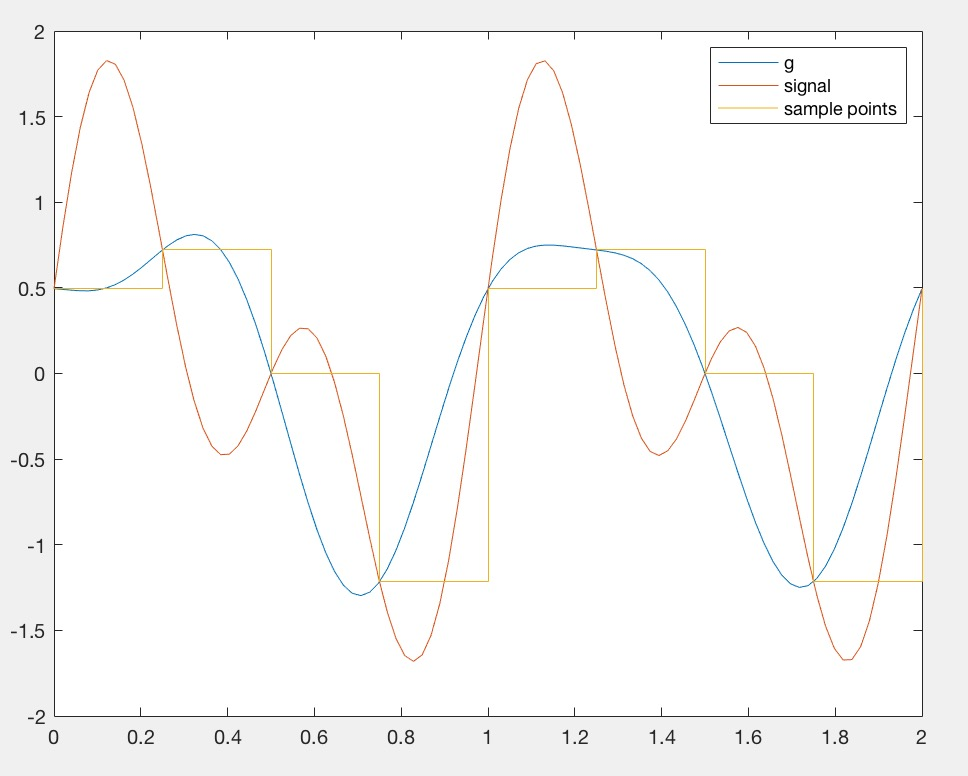
\includegraphics[scale = 0.3]{figures/sinc4}\\
\end{centering}

From the plot we can see that the original and the reconstructed signals match at the points in time where the original signal was sampled. However, since the sampling frequency was rather low (exactly twice the maximum frequency), the reconstruction is far from accurate. For example at time points t=0.3 or t=1.1 we can see large differences. The original signal has a period of 1. Given the interval of 2, we have two full  periods sampled. Our sampled signal is also periodic which means it will repeat itself outside of the intervall. The reconstructed intervall will therefore also be periodic after t=2.

Using a matlab script we noticed, that especially a frequency of $\frac{1}{5}$ worked very well, as seen in the plot below.\\

\begin{centering}
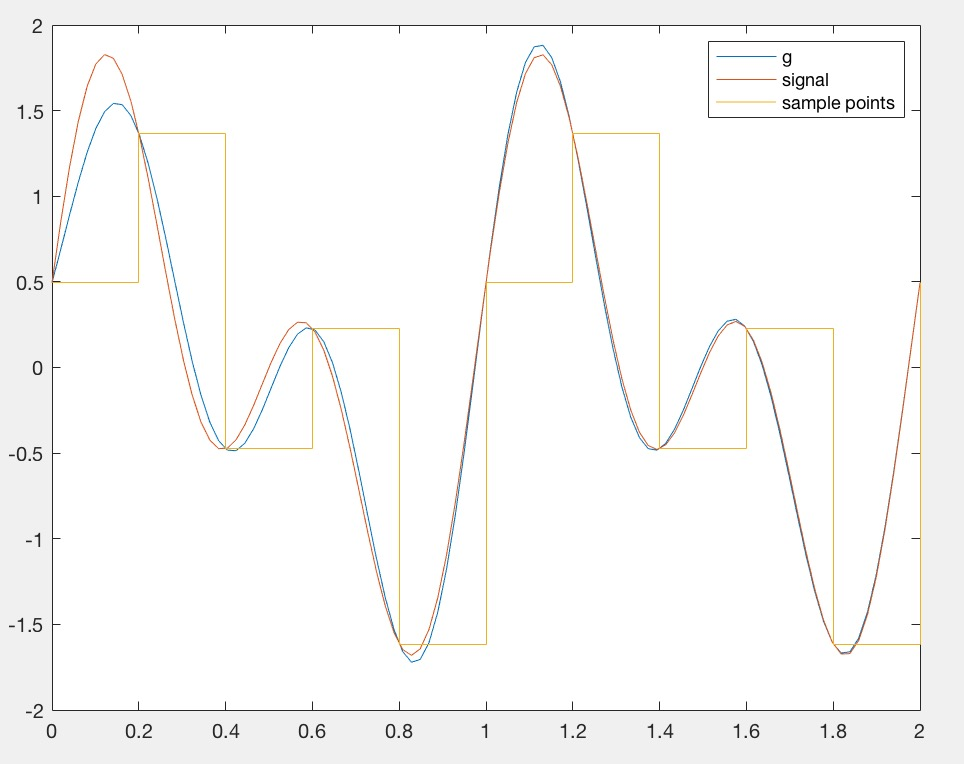
\includegraphics[scale = 0.3]{figures/sinc5}\\
\end{centering}


%	$$\sum_{s=0}^{8} y(t_s) * \frac{sin({4\pi}(t-t_s))}{{4\pi}(t-t_s)}$$
%	$$\sum_{s=0}^{2} y(t_s) * \frac{sin(\frac{4\pi}(t-t_s))}{\frac{\pi}{0.25}(t-t_s)}$$


	\item Simulation using simulink resulted in the following plot of the noisy signal ($e=0.5$)\\
        \begin{centering}
        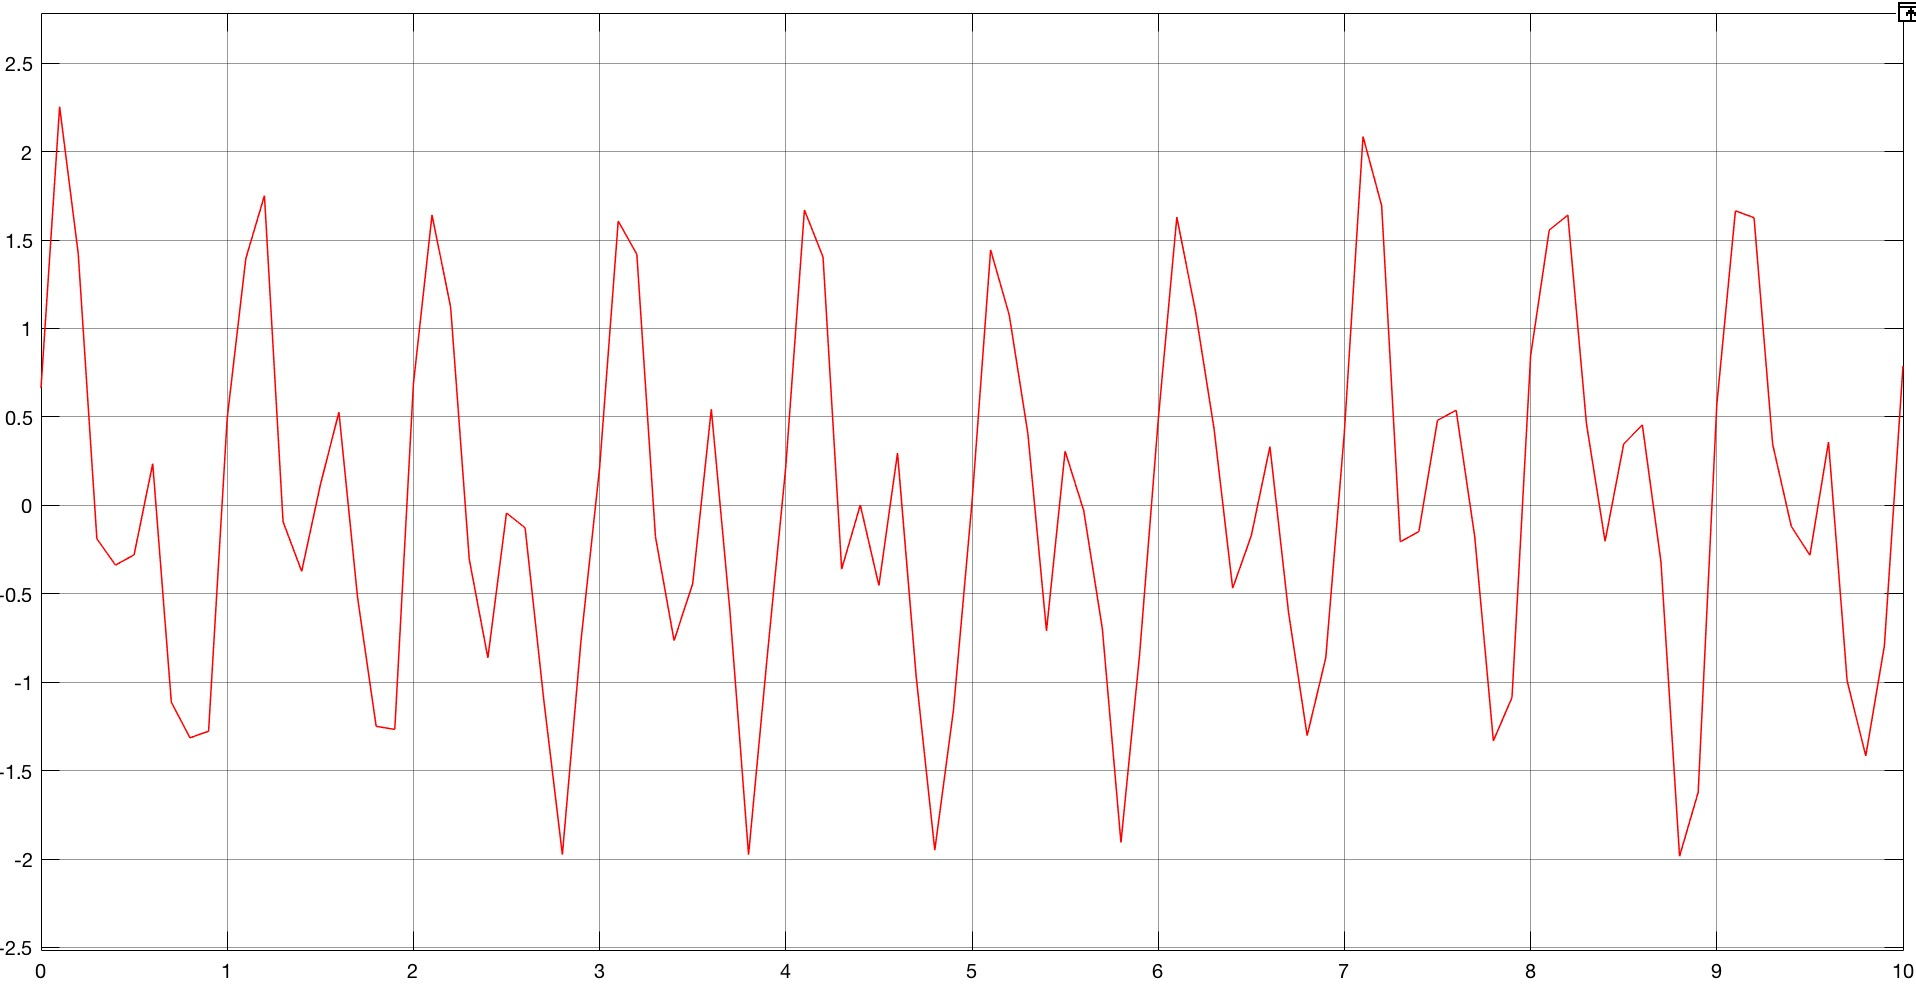
\includegraphics[scale = 0.14]{figures/noise_sim}\\
        \end{centering}

        using the following model:\\
        \begin{centering}
        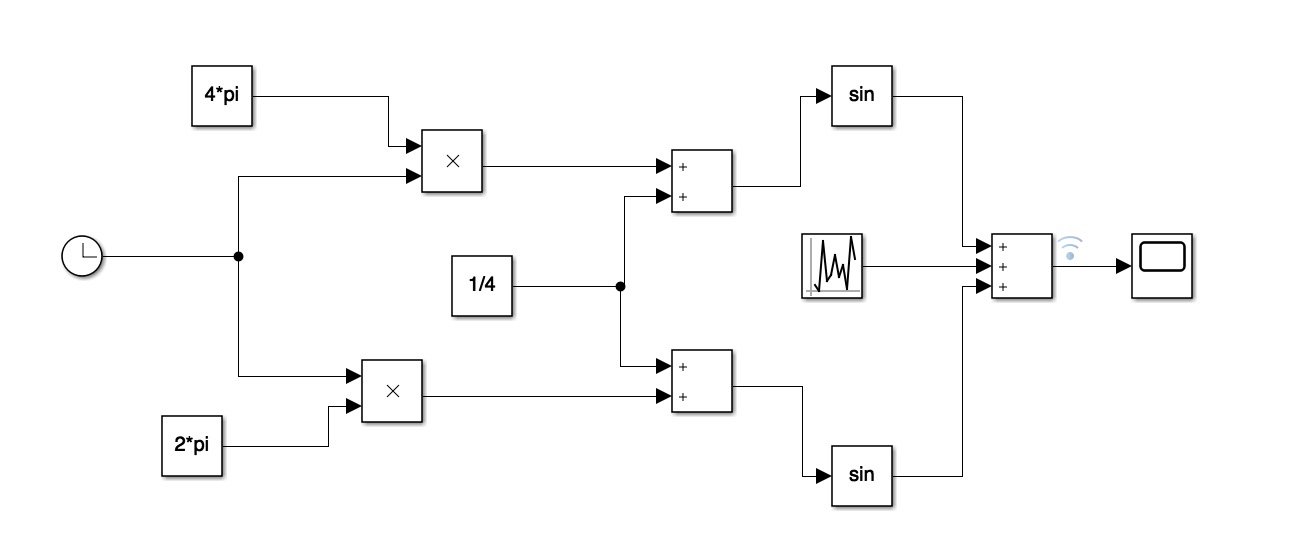
\includegraphics[scale = 0.3]{figures/simulink_1bc}\\
        \end{centering}

	\item Sampling using the same matlab script that we already used for task 1B b) results in the following plots for the f and e values mentioned in the legend.\\
        \begin{centering}
        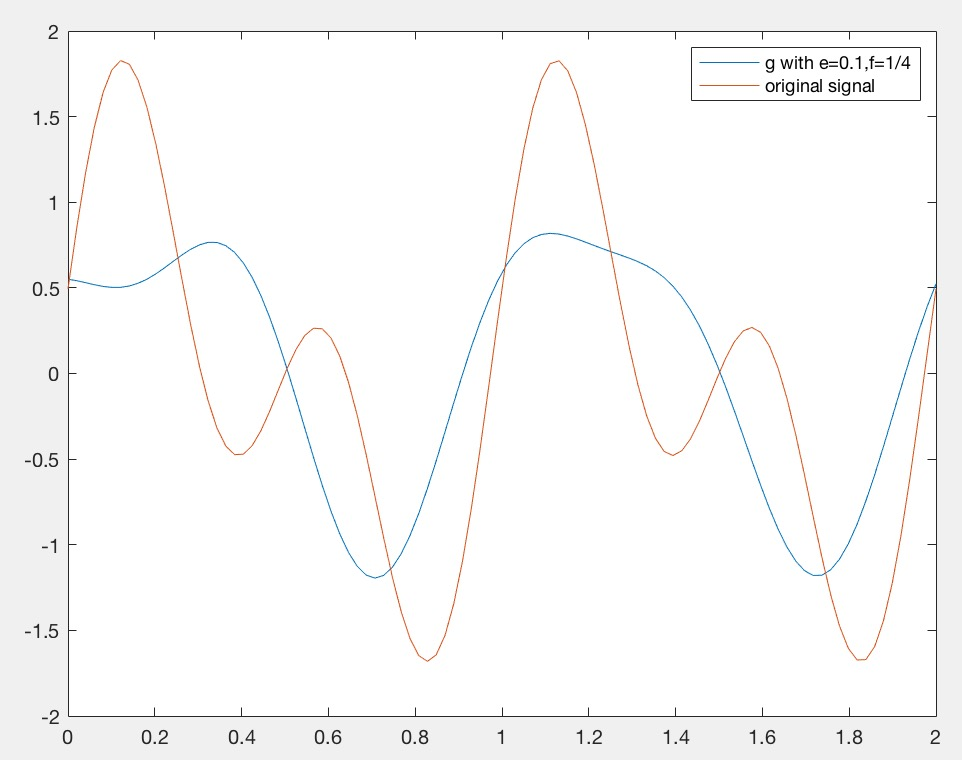
\includegraphics[scale = 0.3]{figures/e01-f14}\\
        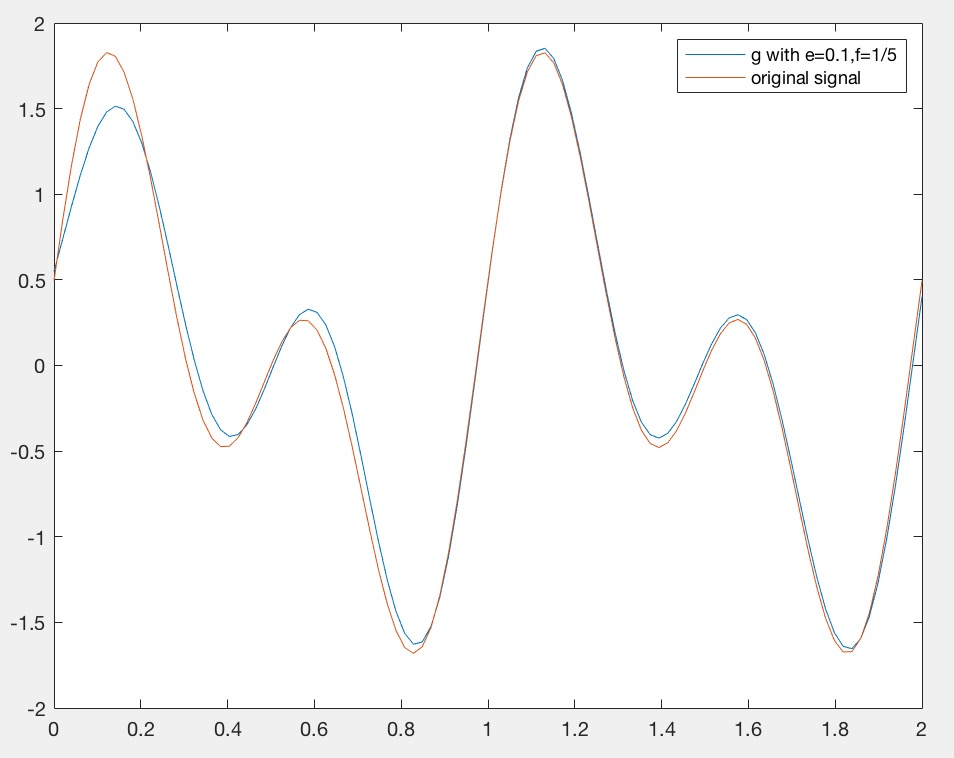
\includegraphics[scale = 0.3]{figures/e01-f15}\\
        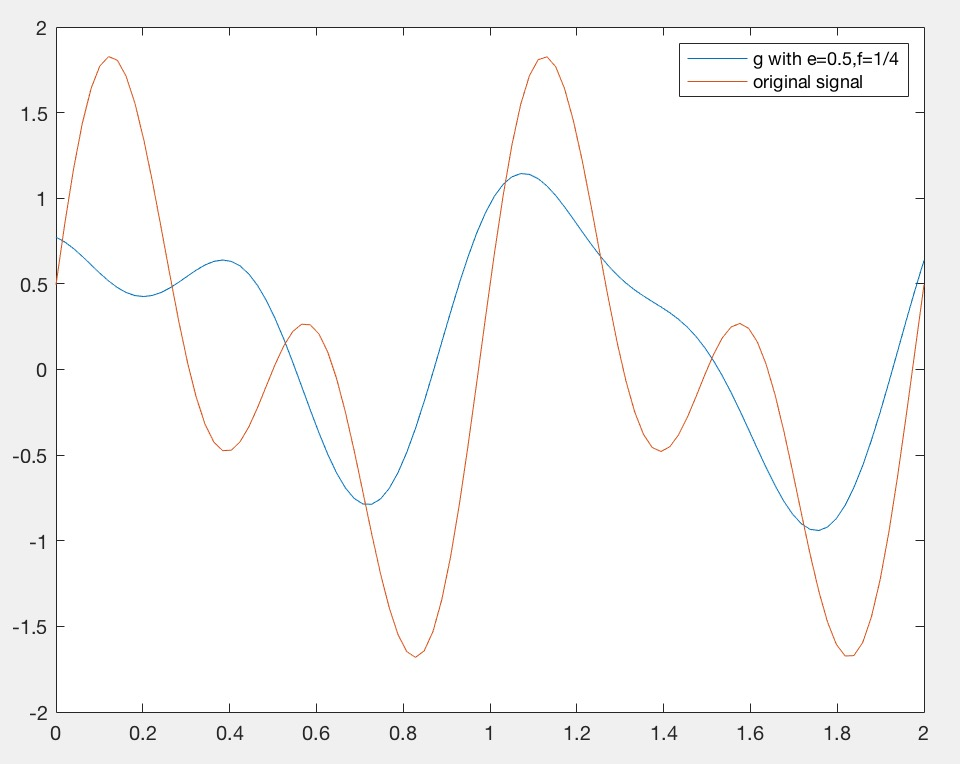
\includegraphics[scale = 0.3]{figures/e05-f14}\\
        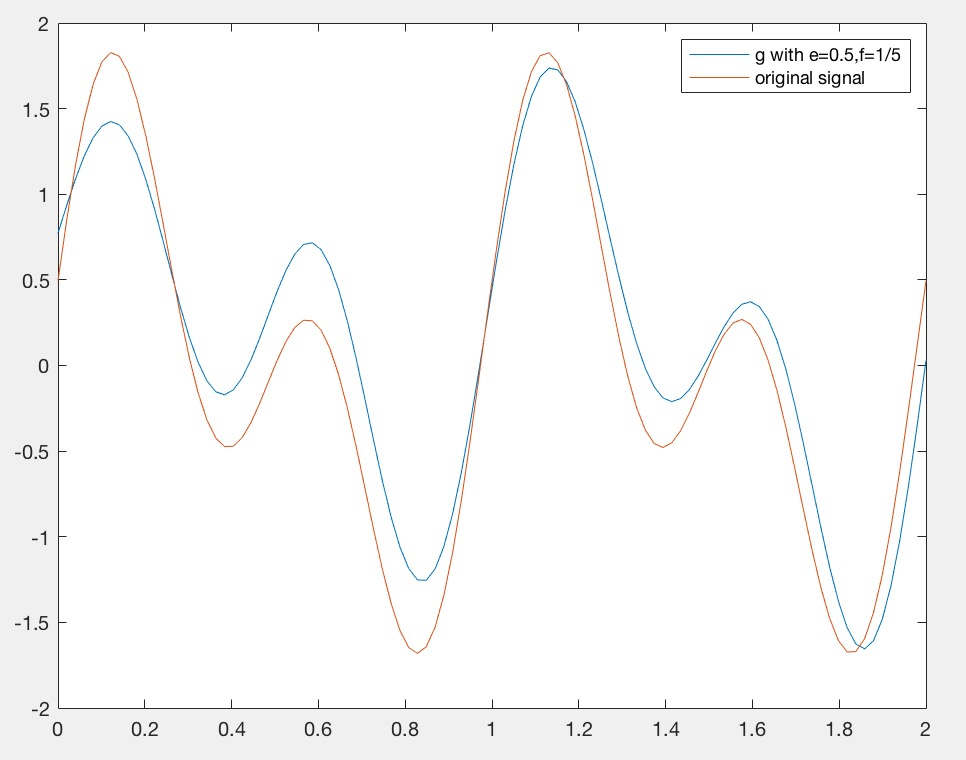
\includegraphics[scale = 0.3]{figures/e05-f15}\\
        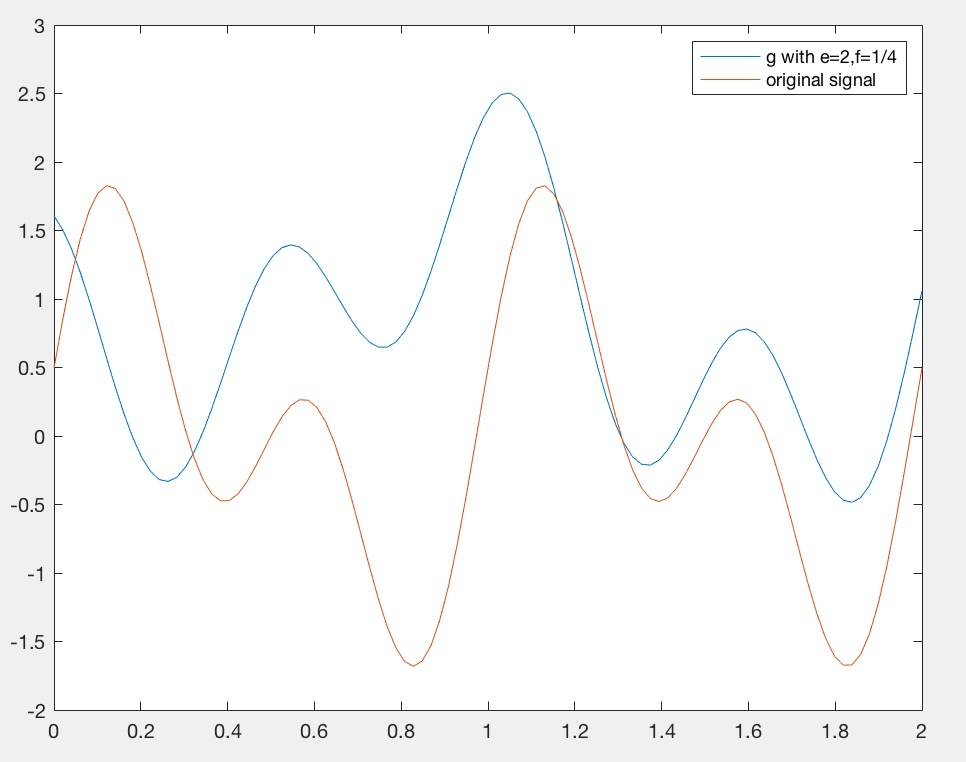
\includegraphics[scale = 0.3]{figures/e20-f14}\\
        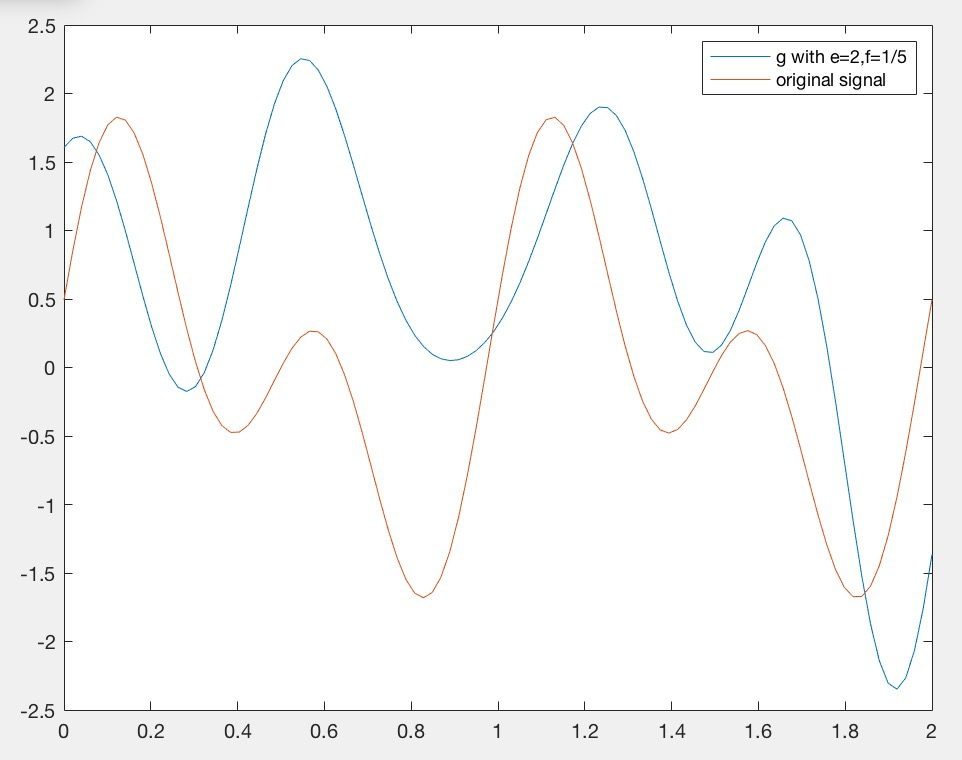
\includegraphics[scale = 0.3]{figures/e20-f15}\\
        \end{centering}

        It is very obvious that the reconstructions gets significantly harder/worse with an higher value of $e$. Additionally there is a very large increase in accuracy when going from sampling frequency $\frac{1}{4}$ to $\frac{1}{5}$.

        % TODO write more?

\end{enumerate}
\section*{Problem B2}
% TODO


\section*{Problem B3}
% TODO


\section*{Problem B4}
\begin{enumerate}[a)]
	\item The integral part of a PID (or PI) controller accumulates the error so far, meaning that the constant error introduced by the bias will accumulate. Since the bias is a function of the wheel velocity, it is constant when the wheel velocity is constant and we want to get rid of that bias. Eventually, by adjusting the integral gain as a response to the accumulation of errors, the error will go to zero. The derivative part of a PID (or PD) controller changes the signal gain based on the error rate of change. Since we have a constant bias, the rate of change will essentially be zero. Therefore a PD controller will have no advantage over simple P controller (only proportional gain), while a PI controller will get rid of the bias and get the error down to zero.\\
Here is our simulink block diagram of the plant and controller:\\
	\item We have two different PID controllers.

	\item TODO
\end{enumerate}

\end{document}
